\documentclass{beamer}
\usetheme{metropolis}
\usepackage[sfdefault]{FiraSans}
\usepackage{pgf}
\usepackage{tikzsymbols}
\usepackage{enumitem}
\usepackage{pgfplots}
\usepackage{tikz}
\usepackage[small]{eulervm}
\usetikzlibrary{arrows,arrows.meta}
\title[]{Attractor dynamics in networks with learning rules inferred from in vivo data}
\subtitle{NBJC Presentation}
\author{Dilawar Singh}
\institute[NCBS] % (optional)
{
  \inst{1}%
  National Center for Biological Sciences Bangalore
}
 
\date[VLC 2015] % (optional)
{\today}
\setbeamertemplate{caption}{\raggedright\insertcaption\par}

\newcommand\Panel[1]{\textbf{(#1)}}

\begin{document}
\maketitle

\begin{frame}
    \frametitle{Attractor dynamics in network}

    \begin{columns}[c]

        \column{0.5\textwidth}

        \includegraphics[width=\columnwidth]{./figures/tikz_hopfield.pdf}

        \column{0.5\textwidth}

        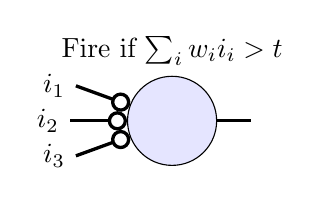
\begin{tikzpicture}[scale=1 , every node/.style={} ]

            \node[circle, draw, inner sep=4mm, fill=blue!10
            , label=Fire if $\sum_i w_i i_i > t$] (nrn) {};

            \foreach \i/\theta in {1/-20,2/0,3/20}
                \draw[o-, very thick] (nrn) -- (\theta:-1.3cm) node[left] {$i_\i$};

            \draw[very thick] (nrn) -- ++(1,0);
            
        \end{tikzpicture}	
    \end{columns}
\end{frame}

% demo frame.
\begin{frame}
    \frametitle{Demo of Hopfield network}

    Number of neurons $k=nm$ where n, m are rows and columns of each pattern.
    Here n=10, m=10 $\implies$ k = 100. 

    \includegraphics[width=\linewidth]{./figures/final_B.png}
    
    \textcolor{red}{\texttt{\$ make demo}}

\end{frame}

\begin{frame}
    \frametitle{Energy landscape of Hopfield network}

    \begin{columns}[c]
        \column{0.5\textwidth}
        
    \includegraphics[width=5cm]{./figures/x536.png}  

    \column{0.5\textwidth}

%    \begin{itemize}
%        \item Attractor: network converges to the stored pattern even when the
%            external inputs are correlated.
%        \item appropriate synaptic connectivity can be generated  through a
%            Hebbian learning process.
%    \end{itemize}
%
    \end{columns}
    \footnote{\url{http://neuronaldynamics.epfl.ch/online/Ch17.S1.html}}
\end{frame}

\begin{frame}
    \frametitle{Are these useful?}

    \begin{columns}[c]
        \column{0.6\textwidth}
        \Cooley
        \begin{itemize}[label=+]
            \small
            \item qualitatively reproduces many experimental observations in
                delayed tasks experiments in monkeys and rodents.
            \item "Selective persistent activity is consistent with attractor dynamics in 
                a recurrent neural network" 
            \item Synaptic connectivity is shaped by experience-dependent
                synaptic plasticity.
        \end{itemize}

        \column{0.5\textwidth}

        \Sey[]
        \begin{itemize}[label=-]
            \small
            \item Patterns (binary images) used are not consistent with data.
            \item Firing rates are bimodal. {\bf Lognormal} is observed in
                performing animals.
                \item Connections are engineered in these networks.
                \item High degree of temporal irregularity in firing of many
                    neuro 
        \end{itemize}
    \end{columns}
\end{frame}

\begin{frame}
    \frametitle{Experimental data}
    \includegraphics[width=0.8\linewidth]{./figures/brunel_presentation_slide20.png}
    \footnote{ \url{https://netadis.files.wordpress.com/2015/06/brunel.pdf}}
\end{frame}

% Now the paper starts.
\begin{frame}
    \frametitle{Learning and retrieval in recurrent neural networks with
    unsupervised Hebbian learning rules}

    \begin{figure}[ht!]
        \centering
        \includegraphics[width=8cm]{figures/fig1.png}
    \label{fig:1}
\end{figure}

\begin{enumerate}[label=(\Alph*)]
    \tiny
\item When a \textbf{novel pattern} is presented to the network,\textbf{synaptic
        inputs} to each neuron in the network ($\xi_i$, for neurons $i$)
        are drawn randomly and independently from a \textbf{Gaussian
        distribution}.  Synaptic inputs elicit firing rates through the static transfer function; i.e., 
        $\phi(\xi_i)$. Some neurons respond strongly (red circles), others weakly (white circles).
    \item The firing rate pattern produced by the synaptic input currents
        modifies the network connectivity according to an \textbf{unsupervised
        Hebbian learning rule}. The connection strength is represented by the
        thickness of the corresponding arrow (the thicker the arrow, the
        stronger the connection).
    \item After learning, a pattern of synaptic inputs that is correlated
        but not identical to the stored pattern is presented to the network.
    \item Following the presentation, the network goes to an attractor
        state that strongly overlaps the stored pattern (compare with A),
        which indicates retrieval of the corresponding memory.
\end{enumerate}
\end{frame}

% figure 2
\begin{frame}
    \frametitle{Inferring Transfer Function and Learning Rule from ITC Data}

    {\small We observe firing rate. Transfer function $\phi$ converts
    firing rates to normally distributed input currents $h_i$. From $h_i$, we
    infer learning rules.}

    \only<1>{
        \begin{columns}[c]
            \column{0.45\textwidth}
            \begin{figure}[ht!]
                \centering
                \includegraphics[width=1.2\columnwidth]{figures/fig2.png}
                \label{fig:2}
            \end{figure}
            {\tiny Each row in top panel represents separate neuron.}

            \column{0.5\textwidth}
            \begin{enumerate}[label=(\Alph*)]
                \tiny
            \item Firing rate distribution w.r.t novel stimuli.  Experimentally recorded (\textcolor{blue}{blue}).
                $\mathcal{N}(1,0)\phi$ where tranfer function \textbf{$\phi: \text{input
                current} \rightarrow \text{Firing rate}$} is from
                {\bf B} (\textcolor{red}{red}). Assumption: input current is sampled
                from Gaussian.
            \item How $\phi$ is computed? Lim et. al., NatNeu. 2015. Later. 
            \item Synaptic plasticity v/s firing rate ($f_r$). 
        \end{enumerate}
    \end{columns}
    }
    
    \only<2>{
        \begin{alertblock}{Estimation of learning rules from $\phi$}
        
        \end{alertblock}

    }
\end{frame}

% figure 3.
\begin{frame}
    \frametitle{Reproducing experimental observation using previous data}

    %{\tiny Dynamics of the Network before, during, and after the Presentation 
    %    of Novel and Familiar Stimuli, Mimicking the Initial Part of a Trial of
    %    a DMS Experiment. 
    %}
    \includegraphics[width=0.8\textwidth]{./figures/fig3.png}

    {\tiny {\bf (A and D, C and F)} Network response to novel (\textbf{A}) and familiar object
        (\textbf{D}). Compare network statistic in (\textbf{C}) and (\textbf{D})
        respectively. \textcolor{blue}{In \Panel{D}, activity does not decay to
        baseline.}

        {\bf (B and E)} Overlap with any stored pattern. In \Panel{B}, novel
        pattern was presented therefore most matches are extremely low.
        \Panel{E} Familiar pattern $m_1$ was presented \textcolor{blue}{blue} match.
    }
    
\end{frame}

% figure 4
% Now the paper starts.
\begin{frame}
    \frametitle{Storage capacity and its dependence on learning rule}

    {\tiny 
    Memory load $\alpha=\frac{\#\text{Stored patterns}}{<\text{connections per neuron}>}$ 

    Learning rule $J_{ij}=f_{ij}g_{ij}$ where J=Synaptic Weight, f=post-synaptic
    component and g is pre-synaptic component. 
    % $f, g: \text{firing rate} \rightarrow \delta J,\;
    $\Delta J_i^k=\frac{Ac_{ij}}{cN}f(r_i^k)g(r_j^k)$, for every novel input $k$.
    }

\begin{figure}[ht!]
    \centering
    \includegraphics[width=8cm]{figures/fig4.png}\label{fig:4}
\end{figure}

\begin{enumerate}[label=(\Alph*)]
    \tiny
    \item In sparse network (low connections per neuron, $\alpha <= 0.4$), 
        we almost always converge to some stored pattern.
    \item Capacity v/s $\beta_g$. Max when $\beta_g =\beta_f$.
    \item Capacity v/s $x_g$. Max when $x_g=x_f$. 
\end{enumerate}
{\tiny $f_i(r)=\frac{\Delta h_i^{fit}(r)}{C^i}=\frac{1}{2}\left[2q_f^i - 1+tanh(\beta_f^i(r-x_f^i))\right]$ }
{\tiny $g_i(r)=\frac{1}{2}\left[2q_g^i - 1+tanh(\beta_g^i(r-x_g^i))\right]$ }

{\footnotesize 
    For good capacity, \textbf{learning rule should be highly non-linear}.
}
\end{frame}

% figure 5.
\begin{frame}
    \frametitle{"Inferred learning rates from the ITC are close to maximizing
    memory storage"}

{\small

    $\Delta J_i^k=\frac{Ac_{ij}}{cN}f(r_i^k)g(r_j^k)$

    $f_i(r)=\frac{\Delta h_i^{fit}(r)}{C^i}=\frac{1}{2}\left[2q_f^i - 1+tanh(\beta_f^i(r-x_f^i))\right]$ 
}

{\tiny $x_f$ (threshold), $\beta_f$ (slope), $q_f$ (offset), $A$ (learning
    rate). 

}
\includegraphics[width=0.75\textwidth]{./figures/fig5.png}

{\tiny 
    f is post-synaptic. g is unconstrained.
}
\end{frame}

% figure 6.
\begin{frame}
    \frametitle{"Chaotic background and retrieval states"}

    {\tiny Chaotic dynamics for some parameter combinations. A=3x of right,
    $\alpha$=0.48. \textbf{On right} For comparison.}

    \begin{columns}[c]
        \column{0.5\textwidth}
        \includegraphics[width=\textwidth]{./figures/fig6.png}\label{fig:6}


        \column{0.5\textwidth}
        \hfill
        \includegraphics[width=0.75\textwidth]{./figures/fig3.png}
    \end{columns}

        {\tiny 
        \Panel{A} Randomly picked 10 neurons. Firing rate before, during, and
        after the presentation of \textbf{familiar} stimulus. \Panel{B} Dynamics of overlap.
        \Panel{C} Overlap v/s $\alpha$. Decays slowly in chaotic case (\tikz
        \node[fill=blue,rectangle,inner sep=2pt] {};) than MFT.
        \Panel{D,E,F} 3 different neurons in 10 different trials. \Panel{G,H,I}
        Slight changes in initial conditions. (G) Complicated distance function
        between two patterns (H) Firing rate (drastic changes). \textbf{Time
        variability in firing patterns!}, and, (I) Overlap
        (roughly same).
    }
\end{frame}

\end{document}
